
%% bare_conf.tex
%% V1.3
%% 2007/01/11
%% by Michael Shell
%% See:
%% http://www.michaelshell.org/
%% for current contact information.
%%
%% This is a skeleton file demonstrating the use of IEEEtran.cls
%% (requires IEEEtran.cls version 1.7 or later) with an IEEE conference paper.
%%
%% Support sites:
%% http://www.michaelshell.org/tex/ieeetran/
%% http://www.ctan.org/tex-archive/macros/latex/contrib/IEEEtran/
%% and
%% http://www.ieee.org/

%%*************************************************************************
%% Legal Notice:
%% This code is offered as-is without any warranty either expressed or
%% implied; without even the implied warranty of MERCHANTABILITY or
%% FITNESS FOR A PARTICULAR PURPOSE! 
%% User assumes all risk.
%% In no event shall IEEE or any contributor to this code be liable for
%% any damages or losses, including, but not limited to, incidental,
%% consequential, or any other damages, resulting from the use or misuse
%% of any information contained here.
%%
%% All comments are the opinions of their respective authors and are not
%% necessarily endorsed by the IEEE.
%%
%% This work is distributed under the LaTeX Project Public License (LPPL)
%% ( http://www.latex-project.org/ ) version 1.3, and may be freely used,
%% distributed and modified. A copy of the LPPL, version 1.3, is included
%% in the base LaTeX documentation of all distributions of LaTeX released
%% 2003/12/01 or later.
%% Retain all contribution notices and credits.
%% ** Modified files should be clearly indicated as such, including  **
%% ** renaming them and changing author support contact information. **
%%
%% File list of work: IEEEtran.cls, IEEEtran_HOWTO.pdf, bare_adv.tex,
%%                    bare_conf.tex, bare_jrnl.tex, bare_jrnl_compsoc.tex
%%*************************************************************************

% *** Authors should verify (and, if needed, correct) their LaTeX system  ***
% *** with the testflow diagnostic prior to trusting their LaTeX platform ***
% *** with production work. IEEE's font choices can trigger bugs that do  ***
% *** not appear when using other class files.                            ***
% The testflow support page is at:
% http://www.michaelshell.org/tex/testflow/



% Note that the a4paper option is mainly intended so that authors in
% countries using A4 can easily print to A4 and see how their papers will
% look in print - the typesetting of the document will not typically be
% affected with changes in paper size (but the bottom and side margins will).
% Use the testflow package mentioned above to verify correct handling of
% both paper sizes by the user's LaTeX system.
%
% Also note that the "draftcls" or "draftclsnofoot", not "draft", option
% should be used if it is desired that the figures are to be displayed in
% draft mode.
%
\documentclass[conference]{IEEEtran}
\usepackage{blindtext, graphicx, caption, color, xcolor}
% Add the compsoc option for Computer Society conferences.
%
% If IEEEtran.cls has not been installed into the LaTeX system files,
% manually specify the path to it like:
% \documentclass[conference]{../sty/IEEEtran}





% Some very useful LaTeX packages include:
% (uncomment the ones you want to load)


% *** MISC UTILITY PACKAGES ***
%
%\usepackage{ifpdf}
% Heiko Oberdiek's ifpdf.sty is very useful if you need conditional
% compilation based on whether the output is pdf or dvi.
% usage:
% \ifpdf
%   % pdf code
% \else
%   % dvi code
% \fi
% The latest version of ifpdf.sty can be obtained from:
% http://www.ctan.org/tex-archive/macros/latex/contrib/oberdiek/
% Also, note that IEEEtran.cls V1.7 and later provides a builtin
% \ifCLASSINFOpdf conditional that works the same way.
% When switching from latex to pdflatex and vice-versa, the compiler may
% have to be run twice to clear warning/error messages.






% *** CITATION PACKAGES ***
%
%\usepackage{cite}
% cite.sty was written by Donald Arseneau
% V1.6 and later of IEEEtran pre-defines the format of the cite.sty package
% \cite{} output to follow that of IEEE. Loading the cite package will
% result in citation numbers being automatically sorted and properly
% "compressed/ranged". e.g., [1], [9], [2], [7], [5], [6] without using
% cite.sty will become [1], [2], [5]--[7], [9] using cite.sty. cite.sty's
% \cite will automatically add leading space, if needed. Use cite.sty's
% noadjust option (cite.sty V3.8 and later) if you want to turn this off.
% cite.sty is already installed on most LaTeX systems. Be sure and use
% version 4.0 (2003-05-27) and later if using hyperref.sty. cite.sty does
% not currently provide for hyperlinked citations.
% The latest version can be obtained at:
% http://www.ctan.org/tex-archive/macros/latex/contrib/cite/
% The documentation is contained in the cite.sty file itself.






% *** GRAPHICS RELATED PACKAGES ***
%
\ifCLASSINFOpdf
  % \usepackage[pdftex]{graphicx}
  % declare the path(s) where your graphic files are
  % \graphicspath{{../pdf/}{../jpeg/}}
  % and their extensions so you won't have to specify these with
  % every instance of \includegraphics
  % \DeclareGraphicsExtensions{.pdf,.jpeg,.png}
\else
  % or other class option (dvipsone, dvipdf, if not using dvips). graphicx
  % will default to the driver specified in the system graphics.cfg if no
  % driver is specified.
  % \usepackage[dvips]{graphicx}
  % declare the path(s) where your graphic files are
  % \graphicspath{{../eps/}}
  % and their extensions so you won't have to specify these with
  % every instance of \includegraphics
  % \DeclareGraphicsExtensions{.eps}
\fi
% graphicx was written by David Carlisle and Sebastian Rahtz. It is
% required if you want graphics, photos, etc. graphicx.sty is already
% installed on most LaTeX systems. The latest version and documentation can
% be obtained at: 
% http://www.ctan.org/tex-archive/macros/latex/required/graphics/
% Another good source of documentation is "Using Imported Graphics in
% LaTeX2e" by Keith Reckdahl which can be found as epslatex.ps or
% epslatex.pdf at: http://www.ctan.org/tex-archive/info/
%
% latex, and pdflatex in dvi mode, support graphics in encapsulated
% postscript (.eps) format. pdflatex in pdf mode supports graphics
% in .pdf, .jpeg, .png and .mps (metapost) formats. Users should ensure
% that all non-photo figures use a vector format (.eps, .pdf, .mps) and
% not a bitmapped formats (.jpeg, .png). IEEE frowns on bitmapped formats
% which can result in "jaggedy"/blurry rendering of lines and letters as
% well as large increases in file sizes.
%
% You can find documentation about the pdfTeX application at:
% http://www.tug.org/applications/pdftex





% *** MATH PACKAGES ***
%
%\usepackage[cmex10]{amsmath}
% A popular package from the American Mathematical Society that provides
% many useful and powerful commands for dealing with mathematics. If using
% it, be sure to load this package with the cmex10 option to ensure that
% only type 1 fonts will utilized at all point sizes. Without this option,
% it is possible that some math symbols, particularly those within
% footnotes, will be rendered in bitmap form which will result in a
% document that can not be IEEE Xplore compliant!
%
% Also, note that the amsmath package sets \interdisplaylinepenalty to 10000
% thus preventing page breaks from occurring within multiline equations. Use:
%\interdisplaylinepenalty=2500
% after loading amsmath to restore such page breaks as IEEEtran.cls normally
% does. amsmath.sty is already installed on most LaTeX systems. The latest
% version and documentation can be obtained at:
% http://www.ctan.org/tex-archive/macros/latex/required/amslatex/math/





% *** SPECIALIZED LIST PACKAGES ***
%
%\usepackage{algorithmic}
% algorithmic.sty was written by Peter Williams and Rogerio Brito.
% This package provides an algorithmic environment fo describing algorithms.
% You can use the algorithmic environment in-text or within a figure
% environment to provide for a floating algorithm. Do NOT use the algorithm
% floating environment provided by algorithm.sty (by the same authors) or
% algorithm2e.sty (by Christophe Fiorio) as IEEE does not use dedicated
% algorithm float types and packages that provide these will not provide
% correct IEEE style captions. The latest version and documentation of
% algorithmic.sty can be obtained at:
% http://www.ctan.org/tex-archive/macros/latex/contrib/algorithms/
% There is also a support site at:
% http://algorithms.berlios.de/index.html
% Also of interest may be the (relatively newer and more customizable)
% algorithmicx.sty package by Szasz Janos:
% http://www.ctan.org/tex-archive/macros/latex/contrib/algorithmicx/




% *** ALIGNMENT PACKAGES ***
%
%\usepackage{array}
% Frank Mittelbach's and David Carlisle's array.sty patches and improves
% the standard LaTeX2e array and tabular environments to provide better
% appearance and additional user controls. As the default LaTeX2e table
% generation code is lacking to the point of almost being broken with
% respect to the quality of the end results, all users are strongly
% advised to use an enhanced (at the very least that provided by array.sty)
% set of table tools. array.sty is already installed on most systems. The
% latest version and documentation can be obtained at:
% http://www.ctan.org/tex-archive/macros/latex/required/tools/


%\usepackage{mdwmath}
%\usepackage{mdwtab}
% Also highly recommended is Mark Wooding's extremely powerful MDW tools,
% especially mdwmath.sty and mdwtab.sty which are used to format equations
% and tables, respectively. The MDWtools set is already installed on most
% LaTeX systems. The lastest version and documentation is available at:
% http://www.ctan.org/tex-archive/macros/latex/contrib/mdwtools/


% IEEEtran contains the IEEEeqnarray family of commands that can be used to
% generate multiline equations as well as matrices, tables, etc., of high
% quality.


%\usepackage{eqparbox}
% Also of notable interest is Scott Pakin's eqparbox package for creating
% (automatically sized) equal width boxes - aka "natural width parboxes".
% Available at:
% http://www.ctan.org/tex-archive/macros/latex/contrib/eqparbox/





% *** SUBFIGURE PACKAGES ***
%\usepackage[tight,footnotesize]{subfigure}
% subfigure.sty was written by Steven Douglas Cochran. This package makes it
% easy to put subfigures in your figures. e.g., "Figure 1a and 1b". For IEEE
% work, it is a good idea to load it with the tight package option to reduce
% the amount of white space around the subfigures. subfigure.sty is already
% installed on most LaTeX systems. The latest version and documentation can
% be obtained at:
% http://www.ctan.org/tex-archive/obsolete/macros/latex/contrib/subfigure/
% subfigure.sty has been superceeded by subfig.sty.



%\usepackage[caption=false]{caption}
%\usepackage[font=footnotesize]{subfig}
% subfig.sty, also written by Steven Douglas Cochran, is the modern
% replacement for subfigure.sty. However, subfig.sty requires and
% automatically loads Axel Sommerfeldt's caption.sty which will override
% IEEEtran.cls handling of captions and this will result in nonIEEE style
% figure/table captions. To prevent this problem, be sure and preload
% caption.sty with its "caption=false" package option. This is will preserve
% IEEEtran.cls handing of captions. Version 1.3 (2005/06/28) and later 
% (recommended due to many improvements over 1.2) of subfig.sty supports
% the caption=false option directly:
%\usepackage[caption=false,font=footnotesize]{subfig}
%
% The latest version and documentation can be obtained at:
% http://www.ctan.org/tex-archive/macros/latex/contrib/subfig/
% The latest version and documentation of caption.sty can be obtained at:
% http://www.ctan.org/tex-archive/macros/latex/contrib/caption/




% *** FLOAT PACKAGES ***
%
%\usepackage{fixltx2e}
% fixltx2e, the successor to the earlier fix2col.sty, was written by
% Frank Mittelbach and David Carlisle. This package corrects a few problems
% in the LaTeX2e kernel, the most notable of which is that in current
% LaTeX2e releases, the ordering of single and double column floats is not
% guaranteed to be preserved. Thus, an unpatched LaTeX2e can allow a
% single column figure to be placed prior to an earlier double column
% figure. The latest version and documentation can be found at:
% http://www.ctan.org/tex-archive/macros/latex/base/



%\usepackage{stfloats}
% stfloats.sty was written by Sigitas Tolusis. This package gives LaTeX2e
% the ability to do double column floats at the bottom of the page as well
% as the top. (e.g., "\begin{figure*}[!b]" is not normally possible in
% LaTeX2e). It also provides a command:
%\fnbelowfloat
% to enable the placement of footnotes below bottom floats (the standard
% LaTeX2e kernel puts them above bottom floats). This is an invasive package
% which rewrites many portions of the LaTeX2e float routines. It may not work
% with other packages that modify the LaTeX2e float routines. The latest
% version and documentation can be obtained at:
% http://www.ctan.org/tex-archive/macros/latex/contrib/sttools/
% Documentation is contained in the stfloats.sty comments as well as in the
% presfull.pdf file. Do not use the stfloats baselinefloat ability as IEEE
% does not allow \baselineskip to stretch. Authors submitting work to the
% IEEE should note that IEEE rarely uses double column equations and
% that authors should try to avoid such use. Do not be tempted to use the
% cuted.sty or midfloat.sty packages (also by Sigitas Tolusis) as IEEE does
% not format its papers in such ways.





% *** PDF, URL AND HYPERLINK PACKAGES ***
%
%\usepackage{url}
% url.sty was written by Donald Arseneau. It provides better support for
% handling and breaking URLs. url.sty is already installed on most LaTeX
% systems. The latest version can be obtained at:
% http://www.ctan.org/tex-archive/macros/latex/contrib/misc/
% Read the url.sty source comments for usage information. Basically,
% \url{my_url_here}.





% *** Do not adjust lengths that control margins, column widths, etc. ***
% *** Do not use packages that alter fonts (such as pslatex).         ***
% There should be no need to do such things with IEEEtran.cls V1.6 and later.
% (Unless specifically asked to do so by the journal or conference you plan
% to submit to, of course. )


% correct bad hyphenation here
\hyphenation{op-tical net-works semi-conduc-tor}


\begin{document}
%
% paper title
% can use linebreaks \\ within to get better formatting as desired
\title{Bangla Handwritten Numeral Recognition Using Directional Pattern}


% author names and affiliations
% use a multiple column layout for up to three different
% affiliations
\author{\IEEEauthorblockN{Sirajus Salekin}
	\IEEEauthorblockA{Islamic University\\ of Technology\\
Email: salekin@iut-dhaka.edu}
\and
\IEEEauthorblockN{Al Shahriar Rubel}
\IEEEauthorblockA{Islamic University\\ of Technology\\
Email: alshahriar@iut-dhaka.edu}
\and
\IEEEauthorblockN{Talha Ibn Aziz}
\IEEEauthorblockA{Islamic University\\ of Technology\\
Email: talhaibnaziz@iut-dhaka.edu}}

% conference papers do not typically use \thanks and this command
% is locked out in conference mode. If really needed, such as for
% the acknowledgment of grants, issue a \IEEEoverridecommandlockouts
% after \documentclass

% for over three affiliations, or if they all won't fit within the width
% of the page, use this alternative format:
% 
%\author{\IEEEauthorblockN{Michael Shell\IEEEauthorrefmark{1},
%Homer Simpson\IEEEauthorrefmark{2},
%James Kirk\IEEEauthorrefmark{3}, 
%Montgomery Scott\IEEEauthorrefmark{3} and
%Eldon Tyrell\IEEEauthorrefmark{4}}
%\IEEEauthorblockA{\IEEEauthorrefmark{1}School of Electrical and Computer Engineering\\
%Georgia Institute of Technology,
%Atlanta, Georgia 30332--0250\\ Email: see http://www.michaelshell.org/contact.html}
%\IEEEauthorblockA{\IEEEauthorrefmark{2}Twentieth Century Fox, Springfield, USA\\
%Email: homer@thesimpsons.com}
%\IEEEauthorblockA{\IEEEauthorrefmark{3}Starfleet Academy, San Francisco, California 96678-2391\\
%Telephone: (800) 555--1212, Fax: (888) 555--1212}
%\IEEEauthorblockA{\IEEEauthorrefmark{4}Tyrell Inc., 123 Replicant Street, Los Angeles, California 90210--4321}}




% use for special paper notices
%\IEEEspecialpapernotice{(Invited Paper)}




% make the title area
\maketitle


\begin{abstract}
%\boldmath
Handwritten character recognition has become a challenging and interesting field in the recent days. It has applications in many fields including reading documents, in hand-held notebooks, touch screens, optical scanning by intelligent systems etc. And thus a lot of research is already done and underway on English alphabets and numerals. On the other hand Bangla being the 5th largest spoken language, has not undergone much research. So we have done a directional pattern approach for feature extraction on Bangla numerals and attained a high accuracy of recognition.

We used LDP(Local Directional Pattern) and GDP(Gradient Directional Pattern) as image pre-processing methods for feature extraction and then the well-known machine learning algorithms KNN and SVM as the classifiers. Then we combined the results to correctly identify the numeral. We used the database CMATERdb 3.1.1 performing a 6-fold cross validation on the 6000 images present to acheive an astounding recognition rate of accuracy 95.62\% without over-fitting the data.
\end{abstract}
% IEEEtran.cls defaults to using nonbold math in the Abstract.
% This preserves the distinction between vectors and scalars. However,
% if the journal you are submitting to favors bold math in the abstract,
% then you can use LaTeX's standard command \boldmath at the very start
% of the abstract to achieve this. Many IEEE journals frown on math
% in the abstract anyway.

% Note that keywords are not normally used for peerreview papers.
\begin{IEEEkeywords}
directional approach, GDP, LDP, KNN, SVM, cross-validation
\end{IEEEkeywords}






% For peer review papers, you can put extra information on the cover
% page as needed:
% \ifCLASSOPTIONpeerreview
% \begin{center} \bfseries EDICS Category: 3-BBND \end{center}
% \fi
%
% For peerreview papers, this IEEEtran command inserts a page break and
% creates the second title. It will be ignored for other modes.
\IEEEpeerreviewmaketitle



\section{Introduction}
Handwriting recognition is a process where a machine tries to interpret images of characters written by hand into what it represents like a numeral or an alphabet. Like in our case to identify which digit of the bangla numerals is in the image. The image might be preprocessed to remove noise and make it fit for feature extraction. Then there are various feature extraction algorithms to bring out the best features for classifiers to work on. And there are well-known classifiers which work on these attained data or features to identify which is which. This whole process encompasses handwritten character recognition.

\subsection{RECENT WORKS}
\textcolor{red}{Although} Bangla Handwritten Character Recognition has not yet been studied as extensively as English Characters, there still are quite a few attempts of classification which are impressive. Most of the papers earlier lacked databases so self-written letters or images of characters were used which lacked the authenticity and variation that a standard database possessed. But that deficit is not present anymore because there are a few standard and well known databases. Some of them are CMATERdb 3.1.1 \cite{cmater} and ISI \cite{isi} which were created respectively in the years 2009 and 2006. Therefore there are quite a few noteworthy papers after 2006. U. Pal et al. in \textcolor{yellow}{2007 \cite{gradientfeature} used} gradient feature to recognize Bengali compound characters. They \textcolor{blue}{did not} use any standard database but \textcolor{blue}{gained} an accuracy of 85.90\% which is quite high for compound characters using 5-fold cross validation. M. Z. Hossain et al. in 2011 \cite{rapidfeature} used rapid feature extraction along with different classifiers and gained an accuracy of 94.12\%.They collected data from 120 writers forming a dataset of 12000 images. Mostly the best classifiers used were Convolution Neural Networks and they gave the most accuracies. In 2016 M. A. H. Akhand et al. \cite{convolution} performed classification of a mixed dataset of Bengali and English numerals using standard databases. The Bangla digits collected from CPVR, ISI \cite{isi} database gave a maximum accuracy of 98.40\% for test sets. Then using autoencoder along with deep convolution neural networking \textcolor{green}{M. Shopon et al.} in 2016 \cite{autoencoder} gave an excellent accuracy of 99.50\% using both CMATERdb 3.1.1 \cite{cmater} and ISI \cite{isi} databases which was the highest accuracy so far. Then in 2017 \cite{blocky} they again performed image augmentation on the CMATER database and gained the accuracy of 99.83\%. More work is being done on Bangla Handwritten character recogntion as days pass.

% needed in second column of first page if using \IEEEpubid
%\IEEEpubidadjcol

% An example of a floating figure using the graphicx package.
% Note that \label must occur AFTER (or within) \caption.
% For figures, \caption should occur after the \includegraphics.
% Note that IEEEtran v1.7 and later has special internal code that
% is designed to preserve the operation of \label within \caption
% even when the captionsoff option is in effect. However, because
% of issues like this, it may be the safest practice to put all your
% \label just after \caption rather than within \caption{}.
%
% Reminder: the "draftcls" or "draftclsnofoot", not "draft", class
% option should be used if it is desired that the figures are to be
% displayed while in draft mode.
%
%\begin{figure}[!t]
%\centering
%\includegraphics[width=2.5in]{myfigure}
% where an .eps filename suffix will be assumed under latex, 
% and a .pdf suffix will be assumed for pdflatex; or what has been declared
% via \DeclareGraphicsExtensions.
%\caption{Simulation Results}
%\label{fig_sim}
%\end{figure}

% Note that IEEE typically puts floats only at the top, even when this
% results in a large percentage of a column being occupied by floats.


% An example of a double column floating figure using two subfigures.
% (The subfig.sty package must be loaded for this to work.)
% The subfigure \label commands are set within each subfloat command, the
% \label for the overall figure must come after \caption.
% \hfil must be used as a separator to get equal spacing.
% The subfigure.sty package works much the same way, except \subfigure is
% used instead of \subfloat.
%
%\begin{figure*}[!t]
%\centerline{\subfloat[Case I]\includegraphics[width=2.5in]{subfigcase1}%
%\label{fig_first_case}}
%\hfil
%\subfloat[Case II]{\includegraphics[width=2.5in]{subfigcase2}%
%\label{fig_second_case}}}
%\caption{Simulation results}
%\label{fig_sim}
%\end{figure*}
%
% Note that often IEEE papers with subfigures do not employ subfigure
% captions (using the optional argument to \subfloat), but instead will
% reference/describe all of them (a), (b), etc., within the main caption.


% An example of a floating table. Note that, for IEEE style tables, the 
% \caption command should come BEFORE the table. Table text will default to
% \footnotesize as IEEE normally uses this smaller font for tables.
% The \label must come after \caption as always.
%
%\begin{table}[!t]
%% increase table row spacing, adjust to taste
%\renewcommand{\arraystretch}{1.3}
% if using array.sty, it might be a good idea to tweak the value of
% \extrarowheight as needed to properly center the text within the cells
%\caption{An Example of a Table}
%\label{table_example}
%\centering
%% Some packages, such as MDW tools, offer better commands for making tables
%% than the plain LaTeX2e tabular which is used here.
%\begin{tabular}{|c||c|}
%\hline
%One & Two\\
%\hline
%Three & Four\\
%\hline
%\end{tabular}
%\end{table}


% Note that IEEE does not put floats in the very first column - or typically
% anywhere on the first page for that matter. Also, in-text middle ("here")
% positioning is not used. Most IEEE journals use top floats exclusively.
% Note that, LaTeX2e, unlike IEEE journals, places footnotes above bottom
% floats. This can be corrected via the \fnbelowfloat command of the
% stfloats package.

\section{DIRECTIONAL PATTERN}
Directional Pattern is as the name indicates, it is a pre-processing algorithm to capture the changes surrounding a specific pixel of an image. Thus the changed value does not only depend it's own data but also that of it's adjacent pixels. It rearranges the values of the raw data and assigns weighted values to each previous location using variances in the data surrounding it. For example it uses different masks or kernels to change the values, and these masks are different for the different directions it focuses on to capture the change in variance. Hence the name 'directional pattern'.

We have used two algorithms of dirctional pattern in our method for recognizing bengali numerals efficiently. These are LDP and GDP.

\subsection{LDP (Local Directional Pattern)}
The LDP method divides the image into various zones and extracts a histogram from each of these zones which are then used for classification.
There are different masks that can be used to record the changes in the data. The masks that we have used are called 'Kirsch' edge masks. These are 8 masks for eight directions that are applied to the image pixel by pixel form left to right for each line in a zone from to top. We can see from the Figure \ref{fig:kirschmask} that each mask is named according to the direction it focuses on and that each direction has different values on the sides depending on what the mask is doing. The centre value is only 0.
\begin{figure}
	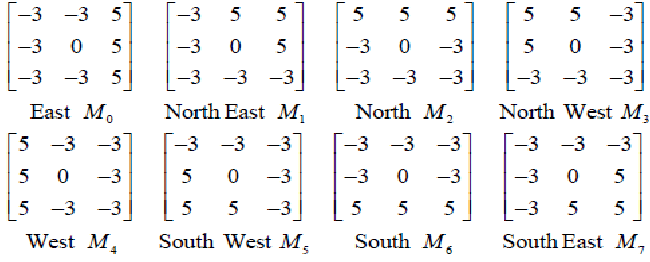
\includegraphics[width=\linewidth]{kirschmask.png}
	\caption{8 Kirsch masks for each direction}
	\label{fig:kirschmask}
\end{figure}
Next for each of the pixels the values gained from applying the mask gives us a matrix of 8 values for each mask which are placed in the 8 directions except the centre. This matrix is then used to assign a binary digit to each of these values. The attained values are sorted and the first k values are assigned 1 and the rest are assigned 0. The value of k can be selected as per need of performance. Using this binary pattern, the number that is formed is placed in the centre. This number is gained by placing each digit serially in the positions they indicate for example - $M_0$ is considered for the LSB or the least significant bit and $M_7$ for the MSB or the most significant bit as shown below. In this way the changed image is attained.
\begin{center}
	All the 8 masks applied and a new matrix formed.\\
\end{center}
\begin{center}
	\begin{tabular}{|c|c|c|}
		\hline
		35 & 123 & 79 \\
		\hline
		16 & 10 & 201 \\
		\hline
		101 & 56 & 99 \\
		\hline
	\end{tabular}
	$\Longrightarrow$mask$\Longrightarrow$
	\begin{tabular}{|c|c|c|}
		\hline
		-738 & -234 & 1094 \\
		\hline
		-914 & X & 902 \\
		\hline
		-746 & -82 & 718 \\
		\hline
	\end{tabular}
\end{center}
\begin{center}
	The attained values form the center value.\\
\end{center}
\begin{center}
	\begin{tabular}{|c|c|c|}
		\hline
		$M_3$ & $M_2$ & $M_1$ \\
		\hline
		$M_4$ & X & $M_0$ \\
		\hline
		$M_5$ & $M_6$ & $M_7$ \\
		\hline
	\end{tabular}
	$\Longrightarrow$
	\begin{tabular}{|c|c|c|}
		\hline
		0 & 0 & 1 \\
		\hline
		0 & X & 1 \\
		\hline
		0 & 0 & 1 \\
		\hline
	\end{tabular}
\end{center}
\begin{center}
	LDP value = $2^0$+$2^1$+0+0+0+0+0+$2^7$ = 131\\
	Thus the center value is replaced by the new value.
\end{center}
\begin{center}
	\begin{tabular}{|c|c|c|}
		\hline
		35 & 123 & 79 \\
		\hline
		16 & 131 & 201 \\
		\hline
		101 & 56 & 99 \\
		\hline
	\end{tabular}
\end{center}

Like this all the values are replaced one by one to finish the pre-processing.

LDP is a robust process which reduces noise and takes variances of data into consideration. Which is why we used LDP as one of the feature extraction processes.

\subsection{GDP (Gradient Directional Pattern)}
GDP is another directional pattern which we used. This is almost the same as LDP except that it works with the gradients of the pixels rather than the grayscale values. In this case before finding the value for the central pixel different kernels are used. The kernel that we used are called 'Sobel' kernels. There are two kernels in 'Sobel' as shown in the Figure \ref{fig:sobelkernel}. Here also we have divided the image into various regions.
\begin{figure}
	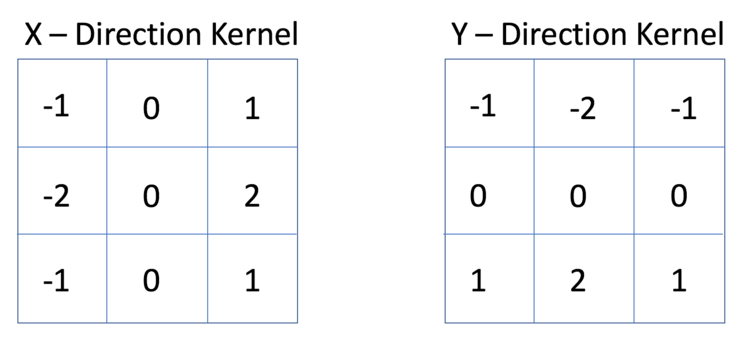
\includegraphics[width=\linewidth]{sobelkernel.png}
	\caption{Sobel Kernels}
	\label{fig:sobelkernel}
\end{figure}
We got two different matrices from applying these two kernels, one along x-axis and another along the y-axis. Then from the two matrices we get the x and y values for each pixel to calculate the gradient and the magnitudes. In our method as we work with direction we have used only the gradient and not the magnitude.
\[magnitude^2 = G_x^2 + G_y^2\]
\[gradient = tan^{-1}(G_y/G_x)\]
Then we have compared the difference of the gradient values with it's adjacent pixel values and placed a 0 if it is greater to a threshold t and 1 if not. This threshold is to be found out by experimenting. The value is usually from $20^0$ to $50^0$. Then we divide the image into regions like before and form a histogram for each region. These histograms are the data to be used for classifiers.
	
GDP is also a pattern which reduces noise like LDP but it is a better feature extraction method than LDP as it works with the  gradient rather than just raw values.

\section{PROPOSED METHOD}
Our proposed method is to use both LDP and GDP to get different vectors. Then use KNN and SVM classifiers on the histograms we obtained and then combine the results like an ensemble method. The 2 steps of our proposed method are briefly explained.
\subsection{Pre-Processing}
We did not perform any noise reduction or any other sort of pre-processing on the images rather we directly used directional pattern feature extraction methods on the images. Even without noise cancellation and slant correction etc. pre-processing methods our proposed method performs excellently giving a high accuracy. We did not normalize the images as we used the whole $32\times32$ bitmap image as the raw data and input for our methods.
We used 2 feature extraction methods - LDP and GDP. The LDP method works on the image to give us a histogram of length 256 for each zone or region each containing the count of the pixel values it represents. Then
these histograms are placed one after another to create a sample vector for classification.\[size of vector = 256 \times number of zones\]
 In case of LDP the zone of $4 \times 4$ gave the best result. And the value of k for sorting was 3 which we used because it gave us most efficiency. The GDP algorithm we used discards the sides of the image so in our case an image of $32 \times 32$ will yield a pre-processed image of $30 \times 30$. For GDP the best result was given by the region division of $6 \times 6$. and for a threshold of 27.5.
\subsection{Classification}
We used two kinds of classifiers to get more accuracy. KNN or K-Nearest Neighbors and SVM or Support Vector Machines for multiple classes. We used KNN and SVM on an image after performing LDP and KNN on the same image after performing GDP.

The KNN considers each value of the vector as a co-ordinate and performs euclidean distance calculation to classify each test sample with respect to each training sample. The value of K=3 for KNN gave best classification. And we used SVM to train each class with respect to every other class using the samples and then we all these classifiers to find the class of each test case. Like this we got 3 different results for the same image. If more than one of the three methods gave the same results then we took that as the final result, otherwise we took the classifier with the most accuracy as the final result which was GDP+KNN.

\section{Experimental Analysis and Discussion}
\subsection{Dataset Creation}
We used the Database CMATERdb 3.1.1 \cite{cmater} which contains 6000 images of bengali numerals. This means for each digit there are 600 images each being bitmap images of size $32 \times 32$. These images are converted into grayscale images and are then pre-processed.
\begin{figure}
	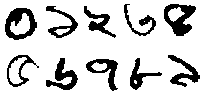
\includegraphics[width=\linewidth]{digits.png}
	\caption{bitmap images of the benagli digits from CMATERdb 3.1.1}
	\label{fig:bangladigits}
\end{figure}

We used k-fold cross validation on the 6000 datasets to create 6 folds each of size 1000. And each time 1 fold acts as test set and the rest 5 folds act as training set. Therefore we focused more on avoiding over-fitting than on accuracy so that the classifier would be more universal, but this decreased the accuracy than some separate datasets created arbitrarily. The highest accuracy attained for the separate folds was 96\% when GDP with t=28.5\% for $6\times6$ zones was applied on the third fold.
\subsection{Result Analysis and Comparison}
We have performed KNN on different zone configurations of GDP and LDP. KNN yields better results on the image when the value of k is odd and the best results are obtained from k=3. As we have shown in Table I the best accuracy is given by LDP performed on region division of $4 \times 4$ which is 93.42\%.
And for k=1 and k=5 also give good rates of recognition compared to 2 and 4.

\begin{center}
	\captionof{table}{Zone-wise accuracy of LDP for KNN}
	\begin{tabular}{cccc}
		\hline
		Classifier & LDP($2\times2$) & LDP($4\times4$) & LDP($8\times8$) \\
		\hline
		KNN (k=5) & 88.3333 & 93.2167 & 92.9833\\
		KNN (k=4) & 87.5500 & 92.7333 & 92.7333\\
		KNN (k=3) & 88.7500 & 93.4167 & 93.2833\\
		KNN (k=2) & 85.2167 & 91.2500 & 91.6667\\
		KNN (k=1) & 88.3333 & 93.2167 & 92.9833\\
		\hline
	\end{tabular}
\end{center}


The $2\times2$ gives an image with 4 regions each giving a histogram of size 256 thus the whole image giving a feature vector of dimensions $4\times256$. Similarly the next two region divisions give feature vectors of sizes respectively $16\times256$ and $64\times254$.
When SVM is performed on the same image after LDP is done, the accuracies are 92.85\% and 92.4333\% respectively for zones $4\times4$ and $8\times8$.
\begin{center}
	\captionof{table}{Zone-wise accuracy of GDP(t=28.5) for KNN}
	\begin{tabular}{cccc}
		\hline
		Classifier & GDP($5\times5$) & GDP($6\times6$) & GDP($10\times10$)\\
		\hline
		KNN (k=5) & 93.17 & 93.90 & 93.88\\
		KNN (k=4) & 91.53 & 93.32 & 93.17\\
		KNN (k=3) & 93.43 & 94.05 & 93.88\\
		KNN (k=2) & 92.52 & 92.22 & 91.98\\
		KNN (k=1) & 93.18 & 93.75 & 93.52\\
		\hline
	\end{tabular}
\end{center}


In Table II we have shown the results of KNN with different values of k performed after GDP is applied with t=28.5 for different zones. The odd values of k give better results than even ones because odd number of results have a better probability of forming a majority while even ones can result in ties and thus decrease classification accuracy. And the zones of $6\times6$ give better recognition rate than all the corresponding zones except for k=4 in which case $5\times5$ is more accurate then $6\times6$.


We have shown the performance of GDP and LDP for different zones in Table III. As expected GDP being a better algorithm than LDP provides better classification accuracy.
\begin{center}
	\captionof{table}{Overall zone-wise Accuracy}
	\begin{tabular}{cccc}
		\hline
		Zones & LDP & Zones & GDP \\
		\hline
		$2 \times 2$ & 88.75 & $5 \times 5$ & 93.43 \\
		$4 \times 4$ & 93.42 & $6 \times 6$ & 94.05 \\
		$8 \times 8$ & 93.28 & $10 \times 10$ & 93.88 \\
		\hline
	\end{tabular}
\end{center}
As we can see more zones and less zones both are reducing the accuracy of the methods although usually more regions give better results. Therefore an optimum number of zones must be selected for the best outcome. In case of LDP the zone is $4 \times 4$ and for GDP it is $6 \times 6$. They respectively divide the image into $8 \times 8$ and $5 \times 5$ pixel areas. And they give accuracies of 93.42\% and 94.05\% respectively when KNN(k=3) is applied.

As a result of combining both LDP and GDP we have got a better accuracy on all the digits. The classifiers used are KNN and SVM together which gives a great accuracy of 95.62\% for cross-fold validation. Table IV shows the best results of the different pre-processing methods.

\begin{center}
	\captionof{table}{Comparison of different methods}
	\begin{tabular}{lc}
		\hline
		Recognition Methods & Accuracy \\
		\hline
		KNN(GDP+LDP) + SVM(LDP) & 95.62\\
		KNN(GDP+LDP) & 94.43\\
		KNN(GDP) & 94.05 \\
		KNN(LDP) & 93.42 \\
		SVM(LDP) & 92.85 \\
		KNN(Basic LBP) & 92.23\\
		SVM(GDP) & 90.47 \\
		\hline
	\end{tabular}
\end{center}

We understood after combining both LDP and GDP that ensemble methods give better results than singular methods. LDP gives an accuracy of 93.42\% and GDP gives a better accuracy of 94.05\%. When GDP and LDP are combined the accuracy increases to 94.43\% which is not much improvement as the results to be combined are derived by the same classifier. For 2 options it is difficult to say which is better. When both gave different results we prioritized GDP over LDP. When SVM is used we get 3 results and a better result as the classifier is different. We also implemented different well-known algorithms like Basic Local Binary Pattern or LBP and used KNN as the classifier. All these methods and their accuracies are shown in Table IV.

All the digits of the bengali numerals are not equally difficult to classify. The rate of recognition depends not only on the algorithms and classifiers also on the confusion between 2 or more classes. The more similar they are the less accurately they can be classified. This means unique classes are easier to classify. Each class has it's unique characteristics but the border between them maybe wide or narrow.
\begin{center}
	\captionof{table}{Digit-wise Classification}
	\begin{tabular}{cccc}
		\hline
		Digit & LDP & GDP & LDP+GDP \\
		\hline
		0 & 98.67 & 99.00 & 98.83\\
		1 & 94.83 & 94.50 & 96.00\\
		2 & 97.50 & 97.67 & 98.17\\
		3 & 92.67 & 93.50 & 95.50\\
		4 & 98.17 & 97.00 & 97.83\\
		5 & 88.33 & 92.00 & 94.00\\
		6 & 86.50 & 87.17 & 90.33\\
		7 & 98.00 & 97.83 & 98.33\\
		8 & 99.00 & 98.83 & 99.00\\
		9 & 88.17 & 83.00 & 88.17\\
		\hline
	\end{tabular}
\end{center}
% The LDP in this table is applied and classified using KNN for k=3 which gives the best value. The GDP is also applied in the same way. The LDP+GDP part is our proposed method and uses 3 results to classify LDP-KNN, GDP-KNN and LDP-SVM. The combination follows majority rule except when all three classifications give different results the GDP-KNN is prioritized as it is the best of these three.
From Table V we can understand that the digits 6 and 9 have lesser accuracy than other digits. And again some digits can be accurately classified like 0, 7 and 8. This is because 6 and 9 are more similar to each other and thus create confusion. And on the other hand 0, 7 and 8 are not similar to any other digit. And the methods LDP and GDP each have their own weaknesses and advantages. That is why we have combined both to give a better result and they cover for each others' weaknesses.


\section{Conclusion}
Directional Pattern has not yet been used for recognizing bengali digits so we proposed the directional approach LDP and GDP and for better results we used both together with the classifiers KNN and SVM.  But these are not the best classifiers. Neural Networks and Genetic approaches give better results when identifying handwritten characters. Therefore this is just a prologue. If these methods are used with better classifiers then it might give promising results. So Directional Approach should be worked on to further improve recognition rate of Bengali handwritten numerals.


% if have a single appendix:
%\appendix[Proof of the Zonklar Equations]
% or
%\appendix  % for no appendix heading
% do not use \section anymore after \appendix, only \section*
% is possibly needed

% use appendices with more than one appendix
% then use \section to start each appendix
% you must declare a \section before using any
% \subsection or using \label (\appendices by itself
% starts a section numbered zero.)
%




% Can use something like this to put references on a page
% by themselves when using endfloat and the captionsoff option.
\ifCLASSOPTIONcaptionsoff
  \newpage
\fi



% trigger a \newpage just before the given reference
% number - used to balance the columns on the last page
% adjust value as needed - may need to be readjusted if
% the document is modified later
%\IEEEtriggeratref{8}
% The "triggered" command can be changed if desired:
%\IEEEtriggercmd{\enlargethispage{-5in}}

% references section

% can use a bibliography generated by BibTeX as a .bbl file
% BibTeX documentation can be easily obtained at:
% http://www.ctan.org/tex-archive/biblio/bibtex/contrib/doc/
% The IEEEtran BibTeX style support page is at:
% http://www.michaelshell.org/tex/ieeetran/bibtex/
%\bibliographystyle{IEEEtran}
% argument is your BibTeX string definitions and bibliography database(s)
%\bibliography{IEEEabrv,../bib/paper}
%
% <OR> manually copy in the resultant .bbl file
% set second argument of \begin to the number of references
% (used to reserve space for the reference number labels box)
\begin{thebibliography}{1}

\bibitem{cmater}
Cheng-Lin Liu and Ching Y. Suen, \emph{"A New Benchmark on the Recognition of Handwritten Bangla and Farsi Numeral Characters"}, Pattern Recognition, Volume 42, Issue 12, December 2009, Pages 3287-3295

\bibitem{genetic}
Nibaran Das, Ram Sarkar, Subhadip Basu, Mahantapas Kundu, Mita Nasipuri, 
Dipak Kumar Basu, \emph{"A genetic algorithm based region sampling for selection of local features in handwritten digit recognition application"}, Applied Soft Computing Volume 12, Issue 5, May 2012, Pages 1592-1606.

\bibitem{lbp}
Tasnuva Hassan, Haider Adnan Khan, \emph{"Handwritten Bangla Numeral Recognition using Local Binary Pattern"}, 2nd International Conference on Electrical Engineering and Information and Communication Technology (lCEEICT) 2015, Jahangimagar University, Dhaka-1342, Bangladesh, 21-23 May 2015

\bibitem{sparse}
H. A. Khan, A. A. Helal, and K.  l.  Ahmed, \emph{"Handwritten bangla digit
recognition using sparse representation classifier"} in  Informatics, Electronics and Vision (ICIEV), 2014 International Conference on 23-24 May 2014, pp. 1-6.

\bibitem{isi}
B.B. Chaudhuri. \emph{"A Complete Handwritten Numeral Database of Bangla – A Major Indic Script"}, Guy Lorette, Tenth International Workshop on Frontiers in Handwriting Recognition, Oct 2006, La Baule (France), Suvisoft, 2006. <inria-00104486>

\bibitem{gradientfeature}
U. Pal, T. Wakabayashi and F. Kimura, \emph{"Handwritten Bangla Compound Character Recognition Using Gradient Feature"}, 10th International Conference on Information Technology (ICIT 2007), Orissa, 2007, pp. 208-213.
doi: 10.1109/ICIT.2007.62

\bibitem{rapidfeature}
M. Z. Hossain, M. A. Amin and H. Yan, \emph{"Rapid feature extraction for Bangla handwritten digit recognition"}, 2011 International Conference on Machine Learning and Cybernetics, Guilin, 2011, pp. 1832-1837.
doi: 10.1109/ICMLC.2011.6017001

\bibitem{convolution}
M. A. H. Akhand, Mahtab Ahmed, M. M. Rahman, (2016). \emph{"Convolutional Neural Network based Handwritten Bengali and Bengali-English Mixed Numeral Recognition"}, I.J. Image, Graphics and Signal Processing (IJIGSP), 8, 40-50.

\bibitem{autoencoder}
M. Shopon, N. Mohammed and M. A. Abedin, e\emph{"Bangla handwritten digit recognition using autoencoder and deep convolutional neural network"}, 2016 International Workshop on Computational Intelligence (IWCI), Dhaka, 2016, pp. 64-68.
doi: 10.1109/IWCI.2016.7860340

\bibitem{blocky}
M. Shopon, N. Mohammed and M. A. Abedin, \emph{"Image augmentation by blocky artifact in Deep Convolutional Neural Network for handwritten digit recognition"}, 2017 IEEE International Conference on Imaging, Vision and Pattern Recognition (icIVPR), Dhaka, 2017, pp. 1-6.
doi: 10.1109/ICIVPR.2017.7890867



\end{thebibliography}


% biography section
% 
% If you have an EPS/PDF photo (graphicx package needed) extra braces are
% needed around the contents of the optional argument to biography to prevent
% the LaTeX parser from getting confused when it sees the complicated
% \includegraphics command within an optional argument. (You could create
% your own custom macro containing the \includegraphics command to make things
% simpler here.)
%\begin{biography}[{\includegraphics[width=1in,height=1.25in,clip,keepaspectratio]{mshell}}]{Michael Shell}
% or if you just want to reserve a space for a photo:

\begin{IEEEbiography}[{\includegraphics[width=1in,height=1.25in,clip,keepaspectratio]{picture}}]{John Doe}
\blindtext
\end{IEEEbiography}

% You can push biographies down or up by placing
% a \vfill before or after them. The appropriate
% use of \vfill depends on what kind of text is
% on the last page and whether or not the columns
% are being equalized.

%\vfill

% Can be used to pull up biographies so that the bottom of the last one
% is flush with the other column.
%\enlargethispage{-5in}




% that's all folks
\end{document}


